%
% file: main.tex
%   by: GDB
% desc: Rstate Paper for DPDNS 2007
%

%\documentclass[times,twocolumn,10pt]{article}
\documentclass[times,twocolumn]{article}
\usepackage{latex8}
\usepackage{pslatex}
\usepackage{url}
\usepackage{verbatim}
\usepackage{graphicx}
\usepackage{graphics}
\usepackage{float}
\usepackage{epsfig}

\newcommand{\displaycodesize}{\footnotesize}

% Some useful macros
% Multiline comments
\long\def\com#1{}

\floatstyle{boxed}
\newfloat{code}{thp}{lop}
\floatname{code}{Code}

\floatstyle{ruled}
\newfloat{listing}{thp}{lop}
\floatname{listing}{Listing}

% Document configuration

%\title{Checkpointing and Migration for Distributed Python Applications}
\title{State Management for Distributed Python Applications}
\author{Gregory D. Benson \\
    Department of Computer Science\\
    University of San Francisco\\
    benson@cs.usfca.edu \\
    \today \\
}

\com{
\renewcommand{\subsection}{\@startsection
  {section}%
  {2}%
  {0mm}%
  {-\baselineskip}%
  {0.5\baselineskip}%
  {\normalfont\largesize\bold}}
}%\com

\begin{document}
%\pagestyle{empty}

\maketitle 
\thispagestyle{empty}

\begin{abstract}

We present a novel state management mechanism that can be used to
capture the complete execution state of distributed Python applications.
This mechanism can serve as the foundation for a variety of
dependability strategies including checkpointing, replication, and
migration. Python is increasingly used for rapid prototyping parallel
programs and, in some cases, used for high-performance application
development using libraries such as NumPy. Building on Stackless Python
and the River parallel and distributed programming environment, we have
developed mechanisms for state capture at the language level. Our
approach allows for migration and checkpointing of applications in
heterogeneous environments. In addition, we allow for preemptive state
capture so that programmers need not introduce explicit snapshot
requests. Our mechanism can be extended to support application or
domain-specific state capture. To our knowledge, this is the first
general checkpointing scheme for Python. We describe our system, the
implementation, and give some initial performance figures.

\end{abstract}

%\vspace{0.10in}
%\noindent
%{\bf Keywords:} Python, distributed programming, state management, %checkpointing, migration


\section{Introduction}
\label{sec:Introduction}

The future of dependable distributed computing will rely on better
integration of fault tolerance mechanisms at all levels of computer
systems. The programming language run-time system is a natural
location for dependability support. In the long-term, new programming
language semantics with replication and failure handling will help
programmers write fault-tolerant software. However, much more research,
development, and experimentation will be required before new languages
are adopted.  Our belief is that using a high productivity language such as Python~\cite{Python} can allow researchers to explore a larger design space when compared to conventional statically-typed languages.

We have developed the \emph{River} framework to facilitate the
development of reliable distributed Python programs and the rapid
prototyping of reliable parallel programming systems. River is
implemented entirely in Python and is based on a few fundamental
concepts that enable the execution of code on multiple virtual machines
and provide a flexible mechanism for communication. These concepts are
supported by the River run-time system, which manages automatic
discovery, connection management, naming, process creation, and message
passing. The simplicity and elegance of the River core combined with
Python's dynamic typing and concise notation make it easy to rapidly
develop distributed applications and a variety of parallel run-time
systems for new programming models. 

%River introduces a novel dynamically
%typed message passing mechanism, called {\it super flexible messaging}
%that makes it easy to send arbitrary data as attribute-value pairs and
%can selectively receive based on matching attribute name and subsets of
%attribute values~\cite{Fedosov:2007:SFM}. This powerful mechanism
%eliminates the need to define a fixed packet structure or specify fixed
%remote interfaces.

% State management

To support different forms of fault tolerance based on state
redundancy~\cite{Gartner:1999:FT} we have developed an integrated state
management mechanism within River. The base mechanism supports
system-level and programmer directed checkpointing for arbitrary River
applications. Thus application-level modifications are not required, but
an explicit interface is provided if the application desires to control
the replication strategy. The base mechanism can be extended to support
various forms of state management, such as memory
exclusion~\cite{Plank:1999:CheckpointExclusion}, incremental
checkpointing~\cite{Plank:1995:Libckpt} or diskless
checkpointing~\cite{Plank:1998:CheckpointDiskless,Chen:2005:CheckpointCoding}.
The River state management facility can be used to support
checkpointing, load balancing, and whole or partial program migration in
clusters and grids. We have implemented our state management support on
top of Stackless
Python~\cite{Tismer:2000:StacklessPython,Stackless:2007}. We use
Stackless Python in an unconventional manner and designed a novel
system-call mechanism to ensure the separation of process state from the
rest of the River system.

% This separation is needed to fully detach
%River process state so that a Stackless tasklet can be pickled.

% GDB: Outline

This paper describes the design and implementation of the state management mechanism we have built in the River programming environment for distributed Python programs.
The rest of this paper is organized as follows.
Section~\ref{sec:Background} provides brief overviews of Python, Stackless Python, and River. 
Section~\ref{sec:Interface} describes the basic River interfaces for state management and some usage scenarios.
Section~\ref{sec:Implementation} details the implementation.
Section~\ref{sec:Experiments} presents the results of some basic experimentation of checkpointing Python applications.
Section~\ref{sec:Conclusions} makes some concluding remarks and gives
directions for future work.

\section{Background}
\label{sec:Background}

\subsection{Python}

Python~\cite{Python} is a high-productivity programming language used in a
wide variety of domains such as web services, program steering, data analysis,
and conventional scripting. It is also widely used for artificial
intelligence, game engines, and scientific computing~\cite{SciPy}. Python's
concise syntax combined with dynamic typing, built-in data structures, and a
rich standard library facilitates rapid program implementation. The language
implementation is also very portable across a variety of processor
architectures and operating systems. However, Python's rich semantics and
interpreted execution incurs run-time overhead. This penalty is often offset
by savings in development time and the use of high-performance C libraries
such as NumPy~\cite{NumPy:2007}. We use Python both for prototyping and
application development.

An import aspect of Python data types is that almost all of them can be easily serialized with the {\it pickle} module.  This module creates a byte stream of a Python object instance which can be {\it unpickled} at a later time.

\subsection{Stackless Python}
\label{sec:StacklessPython}

The standard Python implementation, written in C, is referred to as {\it
CPython}. This implementation executes Python programs by first
compiling all source files into Python bytecode. The bytecode is then
interpreted by the Python run-time system. To support function calls and
method invocation, the run-time system uses the C stack to recursively
call the main interpreter loop. This means that as Python programs
run, their execution state consists of high-level Python object
instances and C activation records. This tight coupling of
architecture-specific state and language objects makes it difficult to
capture the state of a Python program.

Stackless Python~\cite{Stackless:2007, Tismer:2000:StacklessPython} is a modified implementation of CPython that solves the state capture problem by decoupling the C stack from the Python execution stack.  A significant result of this modification is that the execution state of a Python program can be pickled to a byte stream.  This functionality serves as the basis for our distributed state management mechanism.  In addition to decoupling the C stack, Stackless Python also adds language support for cooperative {\it tasklets} and communication between tasklets using {\it channels}.  These features make it possible to support thousands of cooperative execution streams in a single Python instance.

\subsection{River}
\label{sec:River}

River is a Python-based framework for distributed
computing~\cite{River:2007}. River consists of a set of Python classes
that provide a core interface and the underlying run-time system. A
River program consists of one or more {\it virtual resources} (VRs)
that execute on River virtual machines (VMs); see
Figure~\ref{fig:core-execution}. VMs can exist locally or remotely and
VRs are named using UUIDs~\cite{RFC4122}. A VM is simply a Python
interpreter running the River run-time system. An initiating VR can
discover existing VMs and deploy itself or other VRs onto selected VMs.
Once running, VRs communicate with each other using a mechanism called
{\it super flexible messaging} (SFM) for sending and receiving
dynamically typed packets~\cite{Fedosov:2007:SFM}.  SFM makes it easy to send arbitrary data as attribute-value pairs and
selectively receive messages based on matching attribute names and subsets of
attribute values. 
%This powerful mechanism eliminates the need to define a fixed packet structure or specify fixed remote interfaces.  
See Listing~\ref{ex:simple-program} for a minimal River program that discovers available VMs then starts VRs on these VMs.  Each child VR sends a message back to the initiating VR.

\begin{figure}[htb]
\centering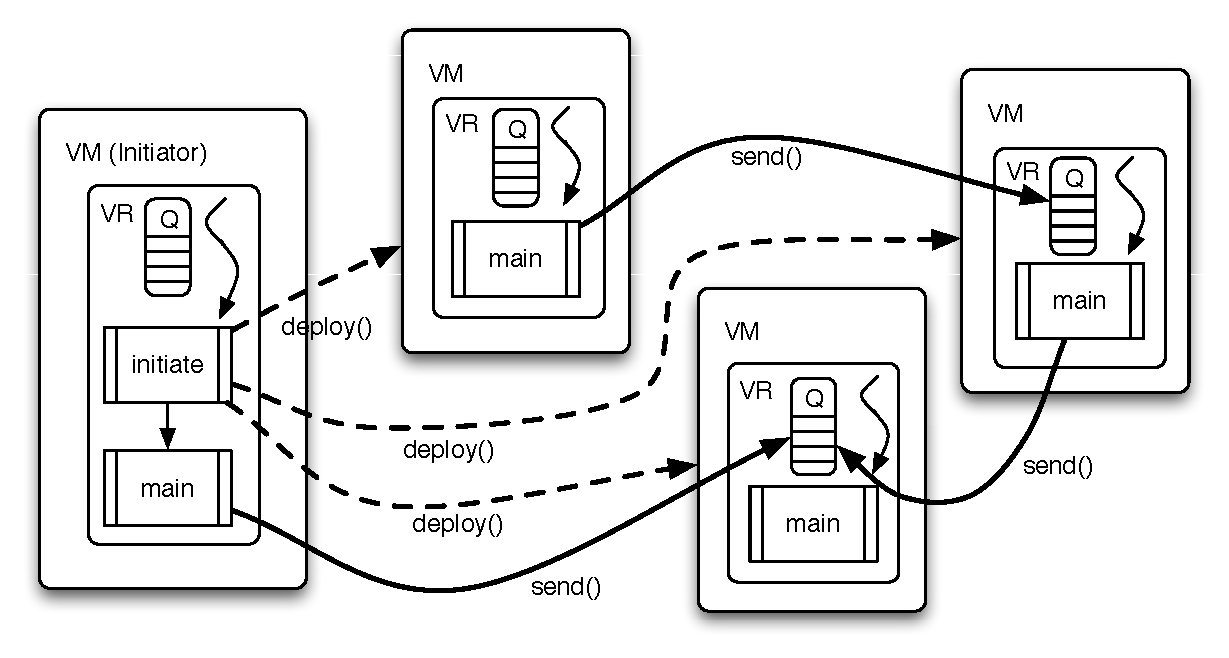
\epsfig{file=core-execution.eps,width=3.3in}
\caption{The Core River Abstractions}\label{fig:core-execution}
\end{figure}


%\begin{figure}[htb]
\begin{listing}
\scriptsize
\begin{verbatim}


from socket import gethostname
from river.core.vr import VR

class Hello(VR):
  def initiate(self):
    discovered = self.discover()
    allocated = self.allocate(discovered)
    deployed = self.deploy(allocated, 
                           module=self.__module__)
    self.vrlist = [vm.uuid for vm in deployed]
    return True

  def main(self):
    if self.parent is None:
      for vr in self.vrlist:
        msg = self.recv(src=vr)
        print '%s says hello' % msg.myname
    else:
      self.send(dest=self.parent, myname=gethostname())
\end{verbatim}
\normalsize
\caption{A Simple River Program}
\label{ex:simple-program}
\end{listing}
%\end{figure}

River was originally conceived with fault-tolerance in mind.  The Core API and underlying programming model supports execution transparency through ``soft'' names via UUIDs and decoupled message queues.  The rest of this paper describes the checkpointing and migration mechanism we have implemented in River.

\section{Interfaces}
\label{sec:Interface}

The River state management mechanism can be used to capture the entire execution
state of a running virtual resource (VR). This state includes all objects
reachable by the containing VR object instance. It also includes all of the
objects reachable from the run-time stack. Optionally, the state of the VR
message queue can also be captured. Capturing the queue is most useful for
consistent distributed state capture. From the programmer's perspective, the VR object
instance serves as a container for all run-time state. The VR object is analogous
to an OS process. The state management facility can be invoked {\it
internally} by an application program in a synchronous fashion or {\it
externally} by a separate utility in an asynchronous fashion.

\subsection{Internal Interface}

For internal usage, the VR interface provides a \verb+snapshot()+ method
to capture program state at the request of the application. In its most
basic form the \verb+target+ parameter specifies a filename to store the
snapshot. In addition, the \verb+exit_vr+ boolean parameter specifies if
the VR should exit or continue executing. Similarly, the \verb+exit_vm+
boolean parameter specifies if the VM should exit or continue running.
This interface allows applications to create checkpoints at regular
intervals or at user prompted points. When a snapshot is restored,
execution begins immediately after the invocation to the
\verb+snapshot()+ method. Restoring the saved state of a single VR can
be done on the command line by passing a \verb+--restore filename+ argument
to \verb+river+, or it can be done externally using a state controller utility.

%\begin{figure}[htb]
\begin{listing}
\scriptsize
\begin{verbatim}


from river.core.vr import VR

class Hello(VR):
  def main(self):
    for i in range(10):
      print i
      if i == 4:
        self.snapshot(target='state_ex.vrst',
                     exit_vr=True, exit_vm=True)
\end{verbatim}
\normalsize
\caption{Simple Usage of Internal State Management}
\label{ex:internalstate}
\end{listing}
%\end{figure}

Listing~\ref{ex:internalstate} shows how to use the \verb+snapshot()+
interface to save the state of the current VR.  This example iterates though a list of integers, saving the state when \verb+i == 4+.  In this example, we exit both the VR and the VM.

%\begin{figure}[htb]
\begin{listing}
\scriptsize
\begin{verbatim}


import cPickle as pickle
from river.core.vr import VR

def state_handler(vrstate):
  vrfile = open('/net/state_ex_cust.vrst', 'w')
  pickle.dump(vrstate, vrfile)
  vrfile.close()

class Hello(VR):
  def main(self):
    for i in range(10):
      print i
      if i == 4:
        self.snapshot(target=state_handler,
                      exit_vr=False, exit_vm=False)
\end{verbatim}
\normalsize
\caption{Internal State Management with State Handler}
\label{ex:internalstatehandler}
\end{listing}
%\end{figure}

The \verb+snapshot()+ interface can be extended by supplying a {\it state handler} function object to the \verb+target+ parameter rather than a string.  In this way, the application can specify precisely what should be done with the snapshot state.  For example, the application may choose to put the state in a specific location on disk, on a network file system, or send the state to a network service.  The handler can also be used to create replicas or to store the state in memory. Listing~\ref{ex:internalstatehandler} shows how to supply a state handler function.

\subsection{External Interface}
\label{sec:ExternalInterface}

River applications can also be manipulated through an external
interface. This interface allows utility programs to pause running VRs,
capture VR state, and restore VR state to available VMs. This interface
can be used to implement full distributed program checkpointing and
migration. We provide a simple state controller utility that performs a
straightforward coordinated checkpoint~\cite{Coti:2006:Checkpointing}.
The utility works by first locating all the VRs associated with a
running application. It then issues pause commands to each VM running an
application VR. Once paused, a message balancing algorithm is used to
ensure all in-flight messages reach their destination VR queues. Note
that the in-flight messages are not processed once received. They are
now considered part of the VR state. Once all messages are balanced, the
VR state on each VM can be captured.  The resulting state can be migrated to idle VMs or collected and written to disk. The VR state can be written in a distributed manner to the local VM file systems or the state of each VR can be collected and combined onto the file system that is associated with the state controller utility.

%\begin{figure}[htb]
\begin{listing}
\scriptsize
\begin{verbatim}


import cPickle as Pickle
from river.core.state import StateClientVR

class save(StateClientVR):
  def main(self):
    vmlist = self.discover(status='*')
    self.pause(vmlist)
    self.balance(vmlist)
    vrcontainer_list = self.getvrs(vmlist)
    vrfile = open(filename, 'w')
    pickle.dump(vrcontainer_list, vrfile)
    vrfile.close()
\end{verbatim}
\normalsize
\caption{Simple Usage of External State Management}
\label{ex:externalstate}
\end{listing}
%\end{figure}

The external state management interface is provided through a special \verb+StateClientVR+ class.  So, state management utilities are also VRs that are given special methods for finding running VMs and VRs and manipulating their state.  Listing~\ref{ex:externalstate} shows a minimal distributed snapshot application using the \verb+StateClientVR+ interface.  A more robust implementation would do more error checking and would not assume that all discovered VMs are a part of the same distributed application.  It is also possible to have each VM save the snapshot state locally rather than collect the state onto a single machine.  This approach can speed up checkpoints by using local disks and eliminate the transfer of state over the network.

\subsection{Extensions}

Both the internal and external state management interfaces are simple but
very flexible.  They can be used to build programming model and
application-specific checkpointing and redundancy.  In addition to these
interfaces, it is also possible to have fine-grain control over state
capture on an object-by-object basis.  Because we utilize the Python
\verb+pickle+ module, programmers can write classes that can determine the state that should be saved for each object using the \verb+getstate()+ and \verb+setstate()+ instance methods.  The \verb+getstate()+ method is called implicitly when an object is being pickled, and likewise, the \verb+setstate()+ method is called implicitly when the serialized snapshot is being unpickled.

%\begin{figure}[htb]
\begin{listing}
\scriptsize
\begin{verbatim}


class LookupTable(object):
    def __init__(self, size):
        self.size = size
        self.fill()

    def fill(self):
        self.table = range(self.size)

    def lookup(self, i):
        return self.table[i]
        
    def __getstate__(self):
        d = {}
        d['size'] = self.size
        return d
        
    def __setstate__(self, d):
        self.size = d['size']
        self.fill()
\end{verbatim}
\normalsize
\caption{Object-specific State Capture}
\label{ex:objectstatecapture}
\end{listing}
%\end{figure}

Listing~\ref{ex:objectstatecapture} shows a simplified \verb+LookupTable+ class that can eliminate state during capture, then recompute the object state when the VR is restored.  The \verb+getstate()+ method simply creates a temporary dictionary with the state to be saved during a snapshot.  In this case we need the \verb+size+ attribute.  The \verb+setstate()+ method restores \verb+size+ and recomputes the table with the \verb+fill()+ method.  This interface can be used to support memory exclusion~\cite{Plank:1999:CheckpointExclusion}.

\subsection{Discussion}

The River state management interface has proven effective at creating arbitrary snapshots of serial and distributed Python programs.  However, the interface currently has two limitations.  First, there is no strict containment of VR state as application VRs and the River run-time system exist in the same execution space.  So, programmers must be sure not to ``pollute'' the VR instance with references to internal River objects.  Similarly, only state reachable via the VR instance will be in the snapshot.  Therefore, global data will not be included unless explicit references from the VR object or descendent objects are made to global objects.  So far, this requirement has not proven to be a significant burden.

The second and more significant limitation concerns I/O modules.  Just as in most other checkpoint systems, open I/O descriptors are troublesome.  This is because open I/O descriptors involve state that exists in the OS and may involve state beyond the local machine in the case of a socket connection.  Most checkpointing systems require applications to reestablish all I/O descriptors once a snapshot has been restored.  We currently take the same approach.  However, we are investigating providing wrapper classes for I/O modules so that certain I/O descriptors can be reestablished in an automated fashion.

\section{Implementation}
\label{sec:Implementation}

This section describes the key implementation details to support state capture of Python programs in River.  We explain the essentials of virtual resource (VR) execution in River and how we decouple VR state from the rest of the River run-time system.  As previously mentioned, we rely on Stackless Python in order to save the execution state of a running Python thread.  We explain how we utilize the Stackless interface to arbitrarily preempt a running VR and capture the VR state.  In order to allow VRs to issue commands to the River run-time system, we introduce atomic {\it system calls} that prevent preemption at undesirable points in execution.  We show how blocking River system calls interact with Stackless execution.  Finally, we describe how we implement distributed checkpointing.

\subsection{River Execution}

As described in Section~\ref{sec:River}, a River program is simply a Python program with a main class that inherits from the VR class.  The River run-time system consists of a Python interpreter and River VM support code.  The resulting execution environment consists of three Python threads: a network thread, a control VR, and the application VR (see Figure~\ref{fig:river-vm}). 

\begin{figure}[htb]
\centering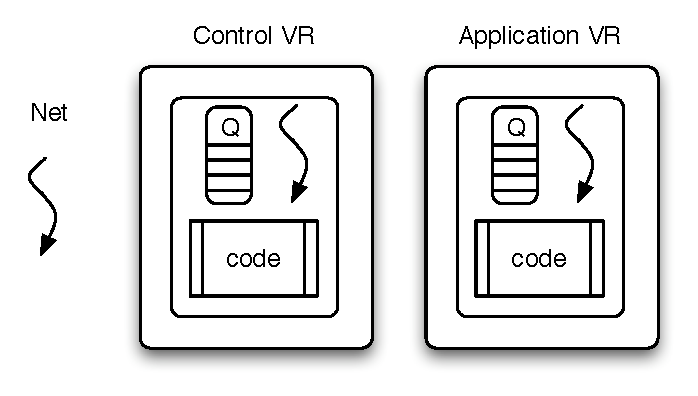
\epsfig{file=river-vm.eps,width=2.5in}
\caption{River VM Execution}\label{fig:river-vm}
\end{figure}

The network thread is used to manage socket-based communication with other River VMs.  The network thread multiplexes connections using the Python \verb+select()+ OS call.  It can handle TCP connections as well as UDP packets for multicast support.  On receipt of a packet, the network thread converts the serialized byte stream to a River message object instance, which is placed in the proper destination VR queue.  The control VR is a special VR that can perform tasks such as allocation and deployment.  The control VR can be extended to handle remote console access and to respond to state control requests.

Application VRs can be specified for launch on the command line or they can be deployed by existing VRs.  While River supports multiple application VRs per River VM, by convention we only run one application VR per River VM because Python does not support true parallel execution of OS threads.

\subsection{Using Stackless Python}

Our state management mechanism utilizes Stackless Python~\cite{Tismer:2000:StacklessPython,Stackless:2007} to capture the arbitrary run-time state of VRs.  As explained in Section~\ref{sec:StacklessPython}, Stackless Python removes the use of the C run-time stack from program execution in the Python interpreter.  This feature combined with the notion of {\it tasklets}, allows dynamic program state to be pickled just as any other Python object instance.  River state management can capture any program that utilizes standard data types and any class that can be pickled.  Exceptions include the array data type and many Python libraries that are wrappers for C libraries.

\subsection{Tasklets and Decoupling VR State}

River can run both on standard CPython and on Stackless Python. Early
implementations existed only for CPython. When running on CPython,
application VRs are executed in the context of a Python thread, which is
mapped to an OS thread. When running River on Stackless Python, the
application VR is executed as a tasklet, which, in turn, is executed in
the context of a Python thread. The host Python thread is referred to as
the {\it main tasklet}. This strategy allows us to control the execution
of the application VR.  

%We can tell Stackless to run a tasklet for a
%given number of Python instructions. After the specified number of
%instructions has executed, control is returned to the main thread. Such
%preemption can be used to see if we should stop execution in order to
%capture the execution state.  

%\begin{figure}[htb]
\begin{listing}
\scriptsize
\begin{verbatim}


self.vr.t = stackless.tasklet(self.vr.main)()

while stackless.getruncount() > 1:
  self.vr.t = stackless.run(1000)
  if self.peek(type='__state__'):
    m = self.recv(type='__state__')
    # Process state messages 'pause' and 'snapshot'
    ...
  if self.vr.t:
    self.vr.t.insert()
  else:
    break
\end{verbatim}
\normalsize
\caption{Executing a VR Tasklet}
\label{ex:vrtasklet}
\end{listing}
%\end{figure}

The code in Listing~\ref{ex:vrtasklet} shows a simplified version of the
main VR tasklet control loop in River.  The key to supporting asynchronous
checkpointing is the ability to preempt the executing VR tasklet.  This
achieved with the \verb+stackless.run(1000)+ method; it tells the
interpreter to execute a specified number of Python bytecodes.  The return
value of \verb+stackless.run()+ is the tasklet that was preempted or finished.  In our case, this will always be the application VR tasklet.  At this point we can see if the VR has received any control messages, such as a {\it pause} request or a {\it snapshot} request.

Running the application VR as a tasklet, then attempting to save
the VR state does not work without careful handling. Notice that the
tasklet is an attribute of the VR object instance. So, to serialize the
VR plus the tasklet, we need to simply pickle the VR instance. The
problem is that when the VR is pickled, the system attempts to
serialize entire state of the VR, the tasklet, and any state {\it
reachable} by these objects. However, the methods provided by the base VR
class have references and make calls into the River VM objects. Because
these objects are reachable through the VR object, serialization results
in an attempt to serialize the entire River VM run-time system.

\begin{figure}[htb]
\centering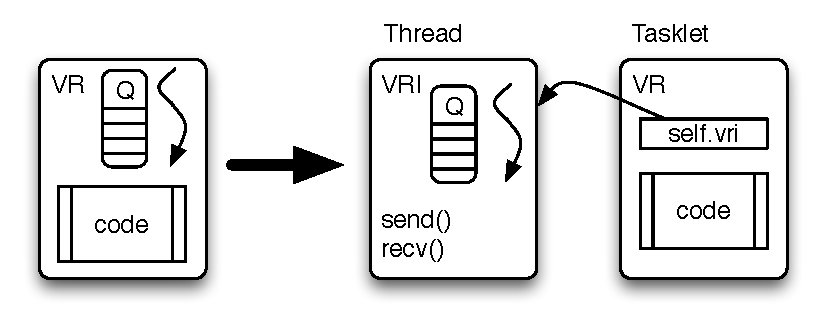
\epsfig{file=river-decoupled-vr.eps,width=3.0in}
\caption{Decoupling VR State}\label{fig:river-decoupled-vr}
\end{figure}

In order to support the serialization of just the application VR state,
we introduce the notion of an {\it internal} VR object, called VRI. The
VRI class contains all of the hard references previously contained in
the VR. Now, only the application supplied state is contained in the VR
object. However, during VR execution we create references to important
{\it system call} methods such as \verb+send()+ and \verb+recv()+. The
references are handled via a single VRI reference (See
Figure~\ref{fig:river-decoupled-vr}). By decoupling system supplied VR
state from application supplied state, we can easily {\it unlink} the
VRI reference when we need to checkpoint the VR.

\subsection{River System Calls}

The base VR class provides methods to discover and allocate remote River VMs as well as to send and receive messages among VR instances.  These methods are implemented in terms of lower-level River VM classes.  We call such methods River {\it system calls} because they require access to the internals of the River run-time system.   While the River system calls do not cross a protection boundary like conventional OS system calls, they do cross a  {\it reference} boundary that introduces River VM runtime references into the call stack of the application VR.  As such, we need to make sure that we do not try to snapshot the state of a VR while it is in the middle of a River system call.

To avoid this River VM reference entanglement, we make all River VM system calls {\it atomic} relative to \verb+stackless.run()+ preemption.
Stackless Python provides an interface to prevent such preemption via the \verb+set_atomic(value)+ tasklet method.  This allows the current tasklet to turn off preemption (\verb+value = True+) or turn it on (\verb+value = False+).  The return value of \verb+set_atomic()+ is the previous atomic state, which allows for recursive atomic sections.

System call atomicity solves one of the problems with preventing
entanglement, but the system calls themselves can introduce references from
the VR object into the River VM.  Therefore, the system calls need to be
{\it soft} references that can be created when we start or resume a VR and
unlinked when we need to snapshot a VR.  We provide system call atomicity
and soft references using Python closures.  For each system call we create
a VR method that points to a closure that performs system calls atomically and ensure that after the atomic operation there are no links from the VR back to the River VM.  

%\begin{figure}[htb]
\begin{listing}
\scriptsize
\begin{verbatim}


def gensyscall_state(self, name):
  def newsyscall(*args, **kwargs):
    t = stackless.current
    curatomic = t.set_atomic( True )
    sysmethod = self.syscalls[name]
    rv = sysmethod(*args, **kwargs)
    del sysmethod
    t.set_atomic( curatomic )
    return rv
  return newsyscall
\end{verbatim}
\normalsize
\caption{System Call Generator}
\label{ex:systemcallgenerator}
\end{listing}
%\end{figure}

The code given in Listing~\ref{ex:systemcallgenerator} is called for
each River system call (e.g., \verb+send()+, \verb+recv()+,
\verb+peek()+, \verb+discover()+, etc.). An important aspect of this code is that the system call is looked up by name in a \verb+syscalls+ table to get a reference.  This allows the system call table to be deleted just before a snapshot is taken.  When a saved VR is restored, we need to populate the system call table just before resuming execution.   Also notice the reference is needed only for the duration of the operation.  After the system call is invoked the reference is removed from the current stack activation record.  This insight did not come immediately.  We initially assumed that the reference would be removed from the stack on return from the wrapper method.  However, it turns out that because preemption can occur between any two bytecodes, we periodically ran into the case where we had completed the system call but not yet returned from the wrapper.  So, in our final solution we do not turn preemption back on until we are certain the reference to the River VM is removed.

The last significant system call implementation issue involves blocking
calls.  Currently, the only blocking call is the \verb+recv()+ call which
blocks the VR while waiting for incoming messages.  We use the same
approach described above for ensuring \verb+recv()+ is atomic relative to
\verb+stackless.run()+ preemption.  However, in order to block, the VR
message queue uses a Python Condition variable.  When new messages arrive,
the VR thread is resumed and the messages can be processed.  In order to
support asynchronous pausing and snapshots, we created special
\verb+__state__+ messages that can only be created by the system.  When the
message queue receives such a message, it returns back to the VR system call wrapper, which then yields the VR tasklet as if it had been preempted.  The VR run loop can then respond to \verb+__state__+ messages.  

\subsection{Saving and Restoring VR State}

With the assurance that the VR state will be decoupled from the VRI state (and the River VM), saving the VR execution state amounts to the following steps:

\begin{enumerate}
\item Create a state container object
\item Remove the VRI reference in the VR
\item Remove system call table (VRI references)
\item Add message queue reference to container
\item Pickle VR (includes the VR tasklet and queue)
\item Add pickled VR to container
\item Add UUID and parent UUID to container
\end{enumerate}

The resulting state container can be pickled and saved to a file or sent over the network.  Restoring the VR state on a VM works in much the same way except the state is extracted from a container and sent to a VM to be restored.

\com{
\begin{enumerate}
\item Read container file
\item Extract saved VR its UUID
\item Allocate a VR on a VM with UUID
\item Send VR state to VM (via ControlVR)
\item Create VRI thread
\item Pass in pickled VR state and queue
\item Unpickle VR state
\item Resume VR tasklet in run loop
\end{enumerate}
}%\com

One implementation detail involving Stackless Python is that tasklets are associated with the thread in which they are created.  It is possible to execute tasklets in multiple Python threads, but tasklet instances cannot move between threads.  This means that a tasklet must be pickled in the thread in which it was created.  Similarly it is necessary to run an unpickled tasklet in the thread in which it was unpickled.  If this restriction is removed in a future version of Stackless Python, it will simplify the River implementation and avoid some extra object copying.

\subsection{Internal State Capture}

Supporting the internal state capture interface amounts to a VR sending a
\verb+__state__+ message to itself.  On receipt of the message, control is
returned to the run loop and the VR state can be saved or, if specified,
the \verb+state_handler+ function can be invoked.  The VR tasklet run loop
will return to executing the VR or exit the VR as specified in the
\verb+__state__+ message.  Similarly, the VM can also be exited if desired,
in which case the VR sends an exit request to the Control VR on the VM.

\subsection{Distributed State Capture}

The external interface for distributed state capture allows an external VR to send control messages to running VRs.  The control messages are sent to the Control VR running on each VM.  The Control VR responds to the following state messages:

\begin{itemize}
\item {\bf pause} Stop the running VR
\item {\bf resume} Continue VR execution
\item {\bf getvr} Retrieve the pickled VR state
\item {\bf deploy} Start a new or saved VR
\item {\bf balance\_counts} Retrieve message counts
\item {\bf balance\_clear} Clear message counts
\end{itemize}

These control messages can be used to implement full distributed
application state capture and full or partial VR migration.  To capture the
entire distributed state we can write a utility VR as outlined in
Section~\ref{sec:ExternalInterface}.  First, we pause all VRs associated
with the application.  Second, we allow in-transit messages to settle.  We
ensure that all messages have reached their destination VRs by querying the
message counts on each VM through the {\bf balance\_counts} control
message.  Full or partial migration can be achieved by pausing all VRs,
balancing messages, then moving the desired VRs.


\section{Experiments}
\label{sec:Experiments}

To demonstrate the usability and overhead of the River state management mechanism we have performed some simple experiments.  First we look at the overhead involved in running serial code within River using Stackless Python.  Second, we look at the cost of serial and distributed checkpointing.  All of the experiments were performed on computers with dual dual-core (4 core) AMD Opteron 270 processors at 2.0GHz and 4 GB of RAM.  We used a Gigabit Ethernet network for the distributed experiments.  The operating system is Linux Fedora Core 5 and we used Python 2.5.1 and Stackless Python 2.5.1.  The machines were used exclusively for these benchmarks.

\subsection{Run-time Overhead}

To quantify the run-time overhead of executing Python code within River with state management support we ran experiments with two programs: the pystone.py (pystone) benchmark from the standard Python distribution and a parallel conjugate gradient solver (congrad) written entirely in Python.  For the Pystone benchmark we ran it for $10^6$ iterations and for the conjugate gradient solver we used an input matrix of size 256 by 265 doubles with 1 processor.

\begin{table} [htb]
\begin{center}
\begin{tabular}{|l|r|r|}  \hline
Version                  &  pystone  &  congrad  \\ \hline\hline
Python                   &    19.14s &    9.56s  \\ \hline
River + Python           &    20.82s &   10.25s  \\ \hline
Stackless Python         &    18.69s &   10.38s  \\ \hline
River + Stackless Python &    21.07s &   10.73s  \\ \hline
\end{tabular}
\end{center}
\caption{River Run-time Performance}
\label{tab:overhead}
\end{table}

Table~\ref{tab:overhead} presents the results of the run-time overhead
experiments.  It is interesting to note that standard Python does worse
than Stackless Python on the pystone benchmark, but does better on the
conjugate gradient solver.  Running the serial code in River + Stackless
adds 13\% overhead to pystone when compared to Stackless alone and 3\%
overhead to congrad for the same comparison.  The River overhead comes from
two sources: additional threads required by the River VM that run
periodically and the tasklet preemption, which currently occurs every 1000
bytecode instructions.  These early results suggest the overhead will not
be prohibitive.

\subsection{Checkpointing Performance}

We have evaluated River checkpointing for serial and distributed operation.  For serial checkpointing we ran the congrad benchmark on a single machine and took checkpoints at different frequencies during execution.  Using the 256 by 256 input matrix the resulting checkpoint file size is 2.7 Mbytes.  Table~\ref{tab:checkpointoverhead} shows the increase in execution time as we increase the number of checkpoints during a run.  For example, 4 checkpoints resulted in 13\% overhead.  With a more practical application, the run times and snapshot sizes would be much larger.  However, the checkpoint frequency for scientific applications would be much lower.  The results here demonstrate that checkpointing for a small Python application using River results in reasonable overhead.

\begin{table} [htb]
\begin{center}
\begin{tabular}{|l|r|r|r|r|}  \hline
\# checkpoints &     0  &       1 &   2    & 4 \\ \hline\hline
congrad        & 10.73s &  11.00s &  11.34s & 12.14s \\ \hline
\end{tabular}
\end{center}
\caption{Serial Checkpoint Overhead}
\label{tab:checkpointoverhead}
\end{table}

For distributed checkpointing we ran the parallel congrad benchmark on a
larger input matrix (1024 by 1024 doubles) across 4 machines.  We started 4
River VMs on each machine.  On another machine in the cluster, we ran an
external asynchronous checkpointing tool similar to the one presented in
Section~\ref{sec:ExternalInterface}.  The tool was configured to take
regular distributed checkpoints at different frequencies.  The resulting
checkpoint files are 26 Mbytes in size.  The checkpoint files where
collected onto a single machine, thus the state needed to be transferred in a linear fashion from each remote VM to a central VM. 

\begin{table} [htb]
\begin{center}
\begin{tabular}{|l|r|r|r|r|}  \hline
\# checkpoints &      0  &       1 &   2    & 4 \\ \hline\hline
congrad        & 202.46s &  212.08s &  219.94s & 236.27s \\ \hline
\end{tabular}
\end{center}
\caption{Distributed Checkpoint Overhead}
\label{tab:dcheckpointoverhead}
\end{table}

Table~\ref{tab:dcheckpointoverhead} show the increasing run time with more frequent checkpoints.  In the worst case with 4 checkpoints the overhead is 17\%.  Note that the checkpoint overhead is much higher than if we checkpointed to the local disk for each VM.


\section{Conclusions and Future Work}
\label{sec:Conclusions}

This paper presents a general mechanism for state management of distributed Python programs.  Our mechanism can be used to implement a wide range of policies for fault tolerance.  While similar mechanisms exist for other languages, this is the first such mechanism for Python programs. 
%Furthermore, the mechanism is quite flexible, so it can be extended or %customized for a particular programming model or application.  
Because we implement checkpointing at the language level, there is no need for underlying operating system support and the mechanism can be used in heterogeneous environments.  We have demonstrated that full-program state capture can be accomplished with reasonable overhead.

In the future we plan to experiment with River state management in the context of higher-level programming models and larger-scale applications.  Furthermore we want to explore supporting native I/O operations and synchronizing checkpoints with disk state.  We believe that the River state management mechanism can be used to rapidly prototype and experiment with different dependability strategies.

\section*{Acknowledgements}

Alex Fedosov developed much of the River core and many of the River
extensions.  Brian Hardie and Tony Ngo worked on the first versions of
the River state management mechanism.


%\pagebreak

%\small
\bibliographystyle{latex8}
\bibliography{river,python,java,mpi,pl,os,networking,hpc,ft}

\end{document}


